\section{NELU: Normalized Gaussian Error Linear Units}\label{sec:method}

Proposition~\ref{prop:no_invariance} showed that no standard self-gated activation can be scale-invariant.
NELU circumvents this impossibility by normalizing the gate's input, decoupling the gate from global scale while remaining in the self-gated form.

%% ============================================================
\subsection{Definition}\label{sec:definition}
%% ============================================================

Given pre-activations $\mathbf{z} \in \mathbb{R}^d$:
\begin{equation}\label{eq:nelu}
    \mathrm{NELU}(\mathbf{z})_i \;=\; z_i \;\Phi\!\left(\frac{z_i}{\operatorname{sg}[\rho]}\right), \quad
    \rho = \operatorname{rms}(\mathbf{z}) = \sqrt{\tfrac{1}{d}\textstyle\sum_j z_j^2}\,,
\end{equation}
where $\Phi(x) = \tfrac{1}{2}[1 + \mathrm{erf}(x/\sqrt{2})]$ is the standard-normal CDF and $\operatorname{sg}[\cdot]$ denotes stop-gradient (treated as constant during backpropagation).
The gate evaluates $z_i / \rho$: the neuron's magnitude \emph{relative to the layer's RMS}, rather than its absolute value.

\begin{verbatim}
def nelu(z, eps=1e-6):
    rms = z.pow(2).mean(-1, keepdim=True).add(eps).sqrt()
    z_hat = z / rms.detach()
    return z * 0.5 * (1 + torch.erf(z_hat / math.sqrt(2)))
\end{verbatim}

When $\rho = 1$, NELU reduces exactly to GELU.
GELU is the special case where pre-activations happen to have unit RMS---the condition under which the standard-normal CDF is a calibrated gate.
No parameters are added.
The same normalization principle applies to any self-gated activation; for example, the SiLU variant is $z_i \cdot \sigma(z_i / \operatorname{sg}[\rho])$.
We focus on GELU as the dominant choice in modern architectures.

%% ============================================================
\subsection{Scale invariance restored}\label{sec:scale_inv}
%% ============================================================

\begin{proposition}\label{prop:homogeneous}
For any $\alpha > 0$: $\mathrm{NELU}(\alpha\mathbf{z}) = \alpha\,\mathrm{NELU}(\mathbf{z})$.
\end{proposition}
\begin{proof}
$\rho(\alpha\mathbf{z}) = \alpha\,\rho(\mathbf{z})$, so $\alpha z_i / \operatorname{sg}[\alpha\rho] = z_i / \operatorname{sg}[\rho]$.
The gate is invariant; the prefactor scales by $\alpha$.
\end{proof}

\begin{corollary}\label{cor:direction}
NELU's output direction is scale-invariant:
$\mathrm{NELU}(\alpha\mathbf{z})/\|\mathrm{NELU}(\alpha\mathbf{z})\| = \mathrm{NELU}(\mathbf{z})/\|\mathrm{NELU}(\mathbf{z})\|$.
\end{corollary}

Scale is not discarded but redirected: removed from the gate (which sees only $\hat{\mathbf{z}}$), preserved in the output magnitude (which scales with $\rho$).
Downstream layers receive scale as gain and pattern as direction---cleanly separated.

\begin{center}
\small
\begin{tabular}{lcccc}
\toprule
 & \textbf{Smooth} & \textbf{Graded gate} & \textbf{No dead neurons} & \textbf{Scale-invariant} \\
\midrule
ReLU   & \texttimes & \texttimes & \texttimes & \checkmark \\
GELU   & \checkmark & \checkmark & \checkmark & \texttimes \\
NELU   & \checkmark & \checkmark & \checkmark & \checkmark \\
\bottomrule
\end{tabular}
\end{center}

NELU is, to our knowledge, the first self-gated activation to appear in the bottom-right cell: smooth, graded, no dead neurons, and scale-invariant.
Figure~\ref{fig:nelu_shape} illustrates: the output magnitude scales with $\rho$, but the gate shape---and therefore the derivative landscape---is invariant.

\begin{figure}[t]
\centering
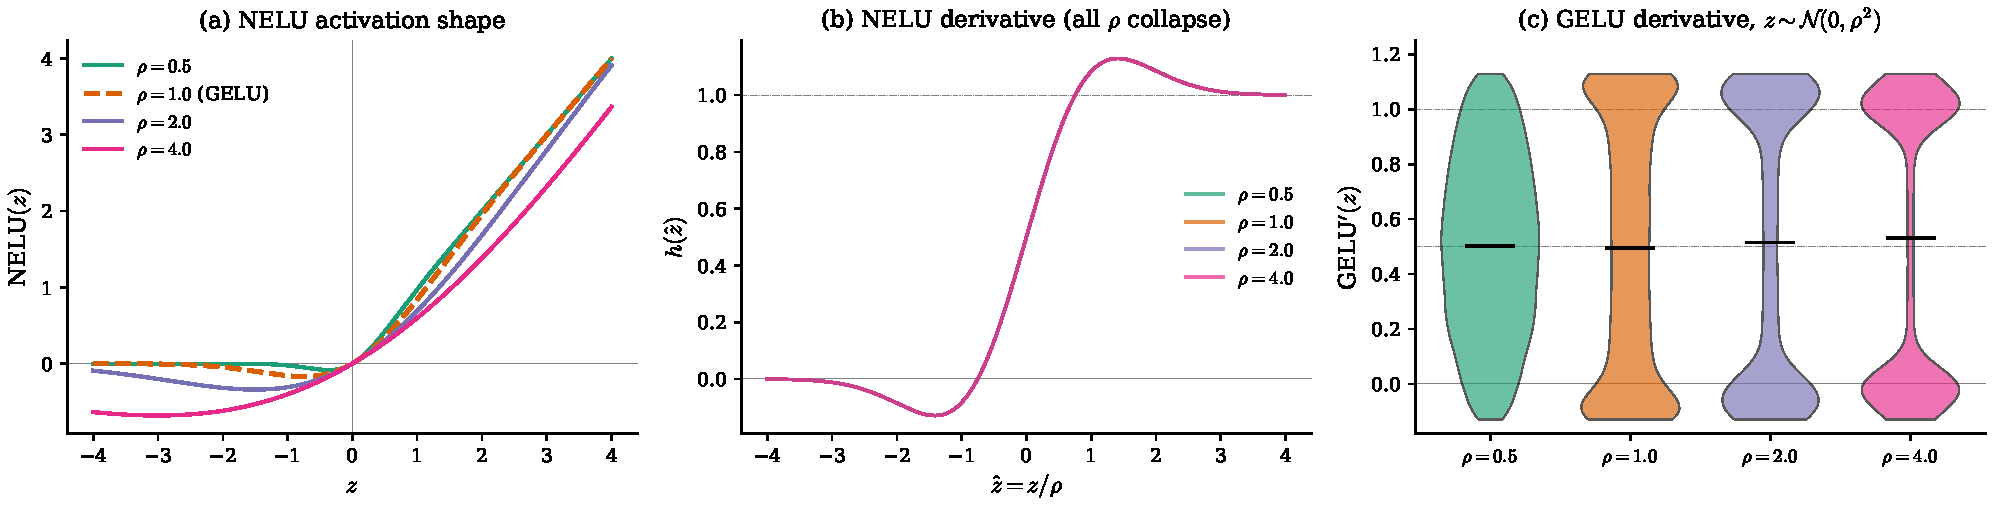
\includegraphics[width=\linewidth]{figures/fig2_nelu_analysis.pdf}
\caption{\textbf{NELU's activation and gradient landscape are scale-invariant; GELU's are not.}
\textbf{(a)}~NELU activation shape for $\rho \in \{0.5, 1, 2, 4\}$. At $\rho{=}1$, NELU $=$ GELU (dashed). The output magnitude scales with $\rho$; the gate shape is invariant.
\textbf{(b)}~NELU's derivative $h(\hat{z}) = \Phi(\hat{z}) + \hat{z}\,\phi(\hat{z})$ as a function of the normalized input $\hat{z} = z/\rho$. All four $\rho$ values collapse to a \emph{single curve}: the gradient landscape is independent of scale.
\textbf{(c)}~GELU's derivative evaluated on inputs drawn from $\mathcal{N}(0, \rho^2)$. At small $\rho$, derivatives spread across $[0, 1]$ (graded regime); at large $\rho$, they collapse to $\{0, 1\}$ (binary regime). The gradient operating point drifts with scale.}
\label{fig:nelu_shape}
\end{figure}

%% ============================================================
\subsection{Mathematical properties}\label{sec:math_properties}
%% ============================================================

Let $\tilde{z}_i = z_i / \rho$ (unit RMS by construction) and $\phi = \Phi'$.

\paragraph{Derivative.}
Under the stop-gradient:
\begin{equation}\label{eq:nelu_deriv}
    h(\tilde{z}_i) \;\equiv\; \frac{\partial\,\mathrm{NELU}(\mathbf{z})_i}{\partial z_i} = \Phi(\tilde{z}_i) + \tilde{z}_i\,\phi(\tilde{z}_i).
\end{equation}
This has the same functional form as GELU's derivative, but evaluated at the normalized value $\tilde{z}_i$.
Because $\tilde{z}_i$ has unit RMS regardless of $\|W\|$, the derivative landscape is independent of weight scale (Figure~\ref{fig:nelu_shape}b,c).

\paragraph{Lipschitz continuity.}
\begin{proposition}\label{prop:lipschitz}
$|h(t)| \leq L$ for all $t \in \mathbb{R}$, where $L = e/\sqrt{2\pi} \approx 1.084$.
\end{proposition}
\begin{proof}
$h'(t) = \phi(t)(2 - t^2)$.
Setting $h'(t) = 0$ gives critical points at $t = \pm\sqrt{2}$.
The global maximum is $h(\sqrt{2}) = \Phi(\sqrt{2}) + \sqrt{2}\,\phi(\sqrt{2}) = e/\sqrt{2\pi}$.
The global minimum is $h(t_{\min}) \approx -0.099$ at $t_{\min} \approx -1.53$.
\end{proof}
GELU shares the same bound, but its operating point drifts with $\|W\|$: at large $\|z\|$, $h \to \{0,1\}$ (binary); at small $\|z\|$, $h \approx 0.5$ (linear); see Figure~\ref{fig:nelu_shape}(c).
NELU always operates at unit-RMS input, maintaining stable gradient statistics throughout training (Figure~\ref{fig:nelu_shape}b).

\paragraph{Boundedness.}
NELU is unbounded above ($\mathrm{NELU}(\mathbf{z})_i \leq z_i$ for $z_i > 0$, with equality at $z_i \to \infty$) and bounded below: $\mathrm{NELU}(\mathbf{z})_i \geq -0.17\,\rho$, since the minimum of $t\,\Phi(t)$ is approximately $-0.17$.

\paragraph{Smoothness.}
Under the stop-gradient, NELU is $C^\infty$ in each $z_i$ for $\rho > 0$, since $\Phi$ is $C^\infty$ and $\rho$ is treated as constant.
The second derivative $h'(t) = \phi(t)(2-t^2)$ is continuous, confirming H\"older continuity with exponent $\alpha \in (1, 2]$.

%% ============================================================
\subsection{Stop-gradient: preserving pointwise learning}\label{sec:gradient}
%% ============================================================

GELU is pointwise: each neuron's gradient depends only on its own pre-activation.
NELU introduces the shared statistic $\rho$; the stop-gradient ensures it does not couple neurons' gradients.

\paragraph{With stop-gradient.}
The Jacobian is diagonal:
\begin{equation}\label{eq:jac_sg}
    \frac{\partial\,\mathrm{NELU}(\mathbf{z})_i}{\partial z_j}\bigg|_{\mathrm{sg}} = \delta_{ij}\,h(\tilde{z}_i).
\end{equation}

\paragraph{Without stop-gradient.}
A rank-one correction appears:
\begin{equation}\label{eq:jac_nosg}
    \frac{\partial\,\mathrm{NELU}(\mathbf{z})_i}{\partial z_j}\bigg|_{\text{no-sg}} = \delta_{ij}\,h(\tilde{z}_i) - \frac{\tilde{z}_j}{d}\,\tilde{z}_i^2\,\phi(\tilde{z}_i),
\end{equation}
coupling neuron $j$'s gradient to all neurons' errors via $\rho$.
The stop-gradient removes this coupling entirely.
Removing it empirically degrades NELU to near-GELU performance (Appendix~\ref{app:ablation}).

%% ============================================================
\subsection{Computational cost}\label{sec:cost}
%% ============================================================

NELU adds one reduction, one sqrt, one detach, and one division---all $O(d)$ and amenable to kernel fusion.
Wall-clock overhead in our unoptimized PyTorch implementation is architecture-dependent (Appendix~\ref{app:overhead}); we expect a fused kernel to close this gap substantially.